\documentclass[12pt]{article}
\usepackage[margin=3cm]{geometry}
\usepackage{blindtext}
\usepackage{chngcntr}
\counterwithin*{section}{part}
\usepackage{enumitem}
\usepackage{listings}
\usepackage{float}
\usepackage{graphicx}
\usepackage{soul}
\usepackage{tikz}
\usepackage{subfig}
\usepackage{hyperref}
\usepackage{amsmath}
\usepackage{multicol}
\usepackage{tcolorbox}
\usepackage{xcolor}
\lstset{language=C++,
    basicstyle=\ttfamily,
    keywordstyle=\color{blue},
    stringstyle=\color{red},
    commentstyle=\color{green},
    morecomment=[l][\color{magenta}]{\#}
}

\hypersetup{
    colorlinks=true,
    linkcolor=blue,
    citecolor=green,
    urlcolor=red
}
\usetikzlibrary{quotes, angles, decorations.markings, intersections}
\usetikzlibrary{calc,patterns,angles,quotes, 3d, intersections, positioning, shapes, automata, positioning}
\newcommand{\tbox}[1]{\noindent\fbox{\parbox{\textwidth}{#1}}}
\title{OS CS219 Notes}
\author{}
\date{\today}

\begin{document}

\maketitle
\setlength{\parskip}{6pt}
\setlength{\parindent}{0pt}

\setlist[itemize]{topsep=0cm,parsep=0cm,itemsep=0cm}
\setlist[enumerate]{topsep=0cm,parsep=0cm,itemsep=0cm}

\noindent\tbox{
    \begin{center}
    \textbf{\Huge Lecture 1}
    \end{center}
}

\section{Introduction}
What is a computer network? A computer network is a group of interconnected devices that can exchange data and resources with each other.
\st{Almost} all of today's devices are in one way or another connect the biggest computer network alias the Internet. There are several 
abstractions and nuances that enable the existence of such a huge structure.

A network consists of several end hosts which are systems that request/receive data using the network. These end hosts are connected 
using links which can directly connect the hosts together or more commonly connect multiple of them to switches/routers which can 
simplify the network while still providing connectivity among hosts. 

\subsection{Topologies}

A group of hosts can be connected in multiple ways. The type of graph that is obtained from considering the 
hosts as nodes and links as edges is called the `topology' of that network. 
Some examples include a bus where all hosts are connected to a common wire. Others include star topology where hosts are connected to a central host. 

Links can also be classified on the basis of how many users can communicate across them.
\begin{itemize}
    \item \textbf{Simplex:} Only one user can talk across a link
    \item \textbf{Duplex:} Both users can communication \textit{simultaneously} across a network. 
    \item \textbf{Half Duplex:} Both users use the same link to communication but not simultaneously. 
\end{itemize}

\begin{figure}
    \centering
    \begin{minipage}{.5\textwidth}
      \centering
      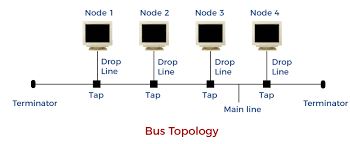
\includegraphics[width=0.9\linewidth]{Diagrams/bus.png}
      \captionof{figure}{Bus Topology}
      \label{fig:test1}
    \end{minipage}%
    \begin{minipage}{.5\textwidth}
      \centering
      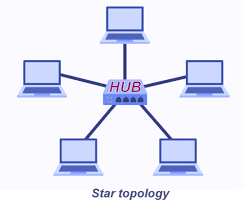
\includegraphics[width=.45\linewidth]{Diagrams/star.png}
      \captionof{figure}{Star Topology}
      \label{fig:test2}
    \end{minipage}
\end{figure}


\subsection{Switch}
What exactly is a switch? The Switch is a network device that is used to segment the networks into different subnetworks called subnets. It can help simplify a 
network by grouping together lots of hosts into a sub-network. A switch has multiple incoming and outgoing links. It is capable of 
routing data from an incoming link to an appropriate outgoing link.

\begin{figure}[H]
    
    \begin{center}
    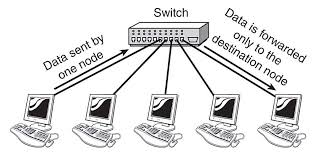
\includegraphics[width = 8cm]{Diagrams/switch.jpeg}
    \end{center}
    \label{fig:switch}
    \caption{Example of a switch}
\end{figure}
\section{Abstractions, Layering in a network}

There is always the possibility to deal with the network as a single structure at once. That is 
to deal with the entire flow of data from the second a request is made by a `user' and all the way till 
the request is serviced in one go. 

However, this is very inconvenient and complicates the network in the sense that any change made to some part of the network can make or break the entire system. 
To combat this the network is clearly split into layers where each layer operates relatively independently and only exposes parts of it that 
are necessary for the higher and lower layers in the network. 

To better understand this let us take an example.

The most common request on the Internet is an HTTP request (ie) a request by a computer for a webpage. Let us see the flow of information when such a request is made.

\begin{enumerate}
    \item \textbf{Application layer:} The URL is entered into a browser and then a user request is made. Then this URL is converted into the \textbf{IP}\footnote{will be dealt with later, assume it is some id for a computer} address of the server
    that holds the page needed by the user. 
    \item \textbf{Transmission layer:} Now that we know the IP address from the application layer, the request for a page is sent to that address using the transmission layer. This layer sends the 
    request message in manageable pieces to the network to be sent to the web server. 
    \item \textbf{Network layer:} Now these `manageable pieces' need to be sent to the destination (ie) web server. The next router/link to which the message is to be sent 
    is decided in this layer. These links `talk' to each other in some sense and know where to send messages to reach the web server. 
    \item \textbf{Data Link layer:} The data link layer deals with splitting the message bit by bit and choosing the appropriate media to transfer them using (ie) Optic fiber, Wireless links etc..
    \item \textbf{Physical layer:} Finally the physical layer deals with transmitting the actual bit signals over whatever media is chosen.
\end{enumerate}


This by no means completely covers the functionality of each layer but rather gives a flavour of each layer's functions. It is easy to see 
how the abstraction is helpful as now the application layer has no need to worry about which media is used to transfer the bits 
and the Physical layer is oblivious to what message it is transferring. 

The abstraction helps to simplify the structure of the network by helping us deal with one subproblem at a time. 



\noindent\tbox{
    \begin{center}
    \textbf{\Huge Lecture 2}
    \end{center}
}


% \section{IP address}

% Each connected device has a unique identifier to describe it.
% This identifier is known as the IP address of a device. 

% The IP address has a hierarchical structure. An example of an IP address is `72.85.5.25'. This can be thought of 
% as being similar to a postal address where the country of your address is the highest level at which location is specified. 
% After this the state, city, area narrow down your location more and the message travels in an organised way from one `level' to another.


% \section{Message}


% A message can be described in various granularities.
% \begin{itemize}
%     \item \textbf{Level 1:} Frame
%     \item \textbf{Level 2:} Symbol
%     \item \textbf{Level 3:} Packet
%     \item \textbf{Level 4:} TCP $\rightarrow$ segment, UDP $\rightarrow$ Datagram
% \end{itemize}


% As we saw in the last Lecture a router has some number of `in' connections and `out' connections which are connected together depending on which 
% `out' connection the message is supposed to be sent. This  `routing' is done by putting each incoming packets on queues corresponding to the outgoing connection we 
% are supposed to send to.

% This rerouting is done so that if the incoming rate to an out connection is greater than its outgoing rate we have the queue as a buffer.


% Why do we just not make the queue very large to prevent these 'drop offs'
% \begin{itemize}
%     \item \textbf{Cost:} Memory is not Free so we need to be aware of the trade offs of increasing the queue size
%     \item \textbf{End-End delay:} If the router has a buffer of say size $Q_{max}$ and an output rate of c $bits/sec$.
%     Now if the queue is almost full and we get a new packet put in at the very end, the packet takes $\frac{Q_{max}}{c}$ time to be put on the next connection. 
%     This is called the End-End delay and clearly a large queue increasing the worst case End-End delay
% \end{itemize}

% The total delay for a transmission of a packet through some K routers would be 
% \[ Delay = \sum_{k = 1}^{k = K}\frac{Q_{max}^k}{c^k} + S_d + T_d\]

% \(S_d\) is called the speed of light delay and \(T_d\) is the transmission delay. 
% In most applications End-End delay is the significant bottle neck for the whole delay. Infact in some applications 
% we prefer dropping packets inorder to not have high delays 

% Most commercial networks have more routers than needed to have good back-ups to prevent the shutdown of their networks even if a router 
% fails. How is this rerouting done?

% \begin{itemize}
%     \item \textbf{Readjusting weights:} The weights of each connection can be adjusted to change the shortest path to the destination
%     \item \textbf{Longest Prefix Match:} There is a router table present which gives us the ID corresponding to a router. When a packet has to make the choice between routers it takes the path with the longest prefix match. 
% \end{itemize}

% \section{Layers of a network}

% \begin{itemize}
%     \item \textbf{L5:} Applications:Web (HTTP), Email (SMTP), Voice Calls (VOIP), Text messaging
%     \item \textbf{L4:} TCP, UDP
%     \item \textbf{L3:} IP (Internet Protocol)
%     \item \textbf{L2:} WiFi, 4G, Bluetooth, Ethernet
%     \item \textbf{L1:} Wireless, Optic Fibre
% \end{itemize}

% \section{Layering and Design Protocols}
% Any subproblem is handled by some protocol.

% We have divided networks into 
% 5 layers. Specifically Application layer, Transmission Layer, Network Layer,Data Link Layer ,Physical Layer.  
% This abstraction enables users to interact only with the layer they are concerned with in that layer without having to deal with the 
% network as a whole. 

% Some advantages of layering networks are:
% \begin{itemize}
%     \item \textbf{Ease of development:} Only certain problems need to be dealt with at each layer
%     \item \textbf{Debugging:} Ease in fixing new problems in each layer independently
%     \item \textbf{Flexibility of Physical technologies, Applications:} As an example whatsapp as an application 
%     only deals with that layer of the network. It doesn't interfere/have to deal with the particular intricacies of the 
%     physical technology used by their users to connect to the network.
%     \item \textbf{Ease of Modification:} We need to change only a particular layer to address problems associated with it. There is no fear of breaking the system due to modifications
%     made to said layer.
%     \item \textbf{Choices at each layer:} Each layer can use multiple media without breaking compatability with the system. 
% \end{itemize}



% \noindent\tbox{
%     \begin{center}
%     \textbf{\Huge Lecture 3}
%     \end{center}
% }



% Disadvantages of layering networks:
% \begin{enumerate}
%     \item There is some opaqueness about other layers. As an example let's say 
%     a packet is sent from a source to destination using a sequence of routers. If a packet is dropped midway, 
%     TCP makes an assumption that they were dropped due to a full queue. Infact there can even be wrong assumptions that a 
%     packet was dropped\footnote{example for another reason is interference in wireless links}. 

%     This mainly arises from the fact that the routers have litte to no communication going with the protocol. 

%     \item There is redundancy at each level of the network. \textbf{TCP} handles retransmission but even \textbf{MAC} handles that. 
%     Let's say that a packet transmission attempt in a wireless link failed. The MAC will make sure that retransmission happens. But this is also taken care by TCP which is redundant.

%     \item Transmission is suboptimal. The sender of the message is unable to specify guarentees they want in the delivery of said packets. This is referred to as a 
%     `Best Effort' system where the network has no guarentees regarding the quality of service
% \end{enumerate}



% \section{Latency Metrics}

% \begin{enumerate}
%     \item \textbf{One-Way delay:} If a packet is sent out at time $t_0$ and it reaches the destination at $t_1$, then the \textit{one way delay} of the packet is $t_1 - t_0$. However measuring 
%     one day delay is difficult since it takes the direct difference in times measured at the source and destination. This difference may drift apart over time due to both systems operating at different clock cycles.
%     \item \textbf{Round-Trip Time:} Once a packet is recieved by the target it sends back an acknowledgment message. The time taken from sending the messages to recieving the acknowledgment is its \textit{round trip time}. 
    
%     \item \textbf{Jitter:} Jitter measures the variability in the latencies associated with the sending some \(k\) packets. Let jitter be \(J\). It can be written as
    
%     \begin{align*}
%     e_k &= |d_{k+1} - d_{k}| \\
%     J &= \frac{1}{n-1} \sum_{k=1}^n e_k 
%     \end{align*}
% \end{enumerate}


% \section{Something I have no idea}

% Imagine a whatsapp message that is being sent across the network. When the message travels from the application layer to the 
\end{document}